\documentclass[11pt,a4paper]{article}
\usepackage[utf8]{inputenc}
\usepackage[T1]{fontenc}
\usepackage[brazil]{babel}
\usepackage{lmodern}
\usepackage[margin=2cm]{geometry}
\usepackage{placeins}
\usepackage{amsmath,amssymb}
\usepackage{booktabs}
\usepackage{graphicx}
\usepackage{hyperref}
\usepackage{xcolor}
\usepackage{titlesec}
\usepackage{tabularx}

% As figuras sao geradas pelo script em RESULTS/project3/. Ajuste os caminhos
% abaixo conforme a organizacao local das figuras (ex.: ao subir no Overleaf,
% basta colocar os PNGs ao lado do .tex ou em uma pasta figuras/).
\graphicspath{{RESULTS/project3/}{figuras/}{./}}

\hypersetup{
    colorlinks=true,
    linkcolor=blue!70!black,
    citecolor=blue!70!black,
    urlcolor=blue!70!black
}

\titleformat{\section}{\large\bfseries}{\thesection.}{0.5em}{}
\titleformat{\subsection}{\normalsize\bfseries}{\thesubsection.}{0.5em}{}
\titlespacing*{\section}{0pt}{1.2ex plus 0.5ex minus .2ex}{0.6ex}
\titlespacing*{\subsection}{0pt}{1.0ex plus 0.4ex minus .2ex}{0.4ex}

\setlength{\parskip}{0.45em}
\setlength{\parindent}{0pt}

\begin{document}

\begin{center}
    {\LARGE \textbf{Projeto 3: Modelo Generativo (VAE) para o Fashion-MNIST}} \\[0.35em]
    {\large Disciplina: Introdução às Redes Neurais Artificiais} \\[0.3em]
    \textbf{Autor:} Henrique Crepaldi (RA: 120410) \\[0.2em]
    \textbf{Código Reprodutível (PyTorch + scikit-learn + Matplotlib):} \url{https://github.com/HCrepaldi/Introduction-to-Artificial-Neural-Networks}
\end{center}
\vspace{-0.5em}
\hrule
\vspace{0.8em}

\section{Objetivo e Formulação do Problema}

O objetivo deste projeto é treinar um \textbf{modelo generativo} para o conjunto de dados \textbf{Fashion-MNIST} (70.000 imagens em tons de cinza, $28 \times 28$ pixels, 10 classes de vestuário) e \textbf{explorar o espaço latente} aprendido. O modelo escolhido é o \textbf{Autoencoder Variacional} (\textit{Variational Autoencoder}, VAE).

Conforme o enunciado, o VAE foi treinado em \textbf{duas configurações de espaço latente} --- \textbf{2 dimensões} e \textbf{8 dimensões} --- e, para cada uma, a melhor topologia foi \textbf{ajustada por otimização de hiperparâmetros guiada pela função de custo no conjunto de validação}. A arquitetura pôde variar livremente entre as duas configurações (a busca escolhe a melhor topologia de forma independente para cada dimensão latente).

\subsection{Por que um VAE, e não um Autoencoder padrão?}
Um autoencoder (AE) padrão aprende uma representação latente \textbf{compacta}, mas o seu espaço latente não é necessariamente \textbf{navegável}: ao amostrar um ponto arbitrário desse espaço e decodificá-lo, podemos obter exemplos inadequados (regiões ``não aprendidas''). O VAE resolve isso \textbf{regularizando} o treino: o termo de divergência de Kullback--Leibler (KL) empurra a distribuição latente para perto de uma Normal padrão $\mathcal{N}(0, I)$, tornando o espaço latente \textbf{contínuo e navegável}. É essa propriedade que faz do VAE um \textit{modelo generativo} de fato: podemos amostrar $z \sim \mathcal{N}(0, I)$ e decodificar para gerar peças de vestuário \textbf{inéditas} e plausíveis (Seção~\ref{sec:geracao}).

\section{O Autoencoder Variacional}

\subsection{Arquitetura}
Tanto o codificador quanto o decodificador são redes \textbf{MLP}. O codificador recebe a imagem achatada ($784$ valores) e, após uma pilha de camadas \texttt{Linear + ReLU}, produz \textbf{dois} vetores de dimensão igual ao espaço latente: a média $\mu$ e o logaritmo da variância $\log\sigma^2$. O decodificador espelha as camadas do codificador e termina em uma \textbf{sigmoide}, de modo que a reconstrução fica em $[0,1]$ --- a mesma escala da entrada normalizada.

\textbf{Por que a rede prevê $\log\sigma^2$ e não $\sigma$ diretamente?} A variância precisa ser positiva. Prevendo o \textbf{logaritmo} da variância, a saída da rede pode assumir qualquer valor real e recuperamos o desvio-padrão de forma sempre positiva e numericamente estável por meio de $\sigma = \exp(\tfrac{1}{2}\log\sigma^2)$.

\subsection{O Truque da Reparametrização}
\label{sec:reparam}
O coração do VAE é a amostragem $z \sim \mathcal{N}(\mu, \sigma^2)$ no gargalo da rede. O problema é que \textbf{essa amostragem é estocástica e não-diferenciável}: ao aplicar a regra da cadeia para calcular os gradientes do erro (reconstrução + KL) em relação aos pesos do codificador, o fluxo do gradiente \textbf{trava} no nó de amostragem de $z$ --- não há como derivar ``através'' de um sorteio aleatório.

A solução é o \textbf{truque da reparametrização}: em vez de sortear $z$ diretamente da distribuição que depende dos parâmetros, movemos a aleatoriedade para um ramo lateral. Sorteia-se um ruído \textbf{padrão} $\varepsilon \sim \mathcal{N}(0, I)$, que não depende de nenhum peso, e monta-se:
\begin{equation}
    z = \mu + \sigma \odot \varepsilon, \qquad \varepsilon \sim \mathcal{N}(0, I).
\end{equation}
Agora $z$ é uma função \textbf{determinística e diferenciável} de $\mu$ e $\sigma$ (com $\partial z/\partial\mu = 1$ e $\partial z/\partial\sigma = \varepsilon$). A única fonte de aleatoriedade, $\varepsilon$, entra como uma constante sem gradiente, de forma que a retropropagação volta a fluir normalmente para o codificador. No código, isso corresponde ao método \texttt{VAE.reparametrizar}.

\subsection{Função de Custo (ELBO)}
A função de custo do VAE combina dois termos:
\begin{equation}
    \mathcal{L} = \underbrace{\mathcal{L}_{\text{rec}}(x, \hat{x})}_{\text{reconstrução}}
    \; + \; \beta \cdot \underbrace{\mathrm{KL}\!\left(\mathcal{N}(\mu, \sigma^2)\,\|\,\mathcal{N}(0, I)\right)}_{\text{regularização}}.
\end{equation}
O \textbf{termo de reconstrução} mede a fidelidade da reconstrução; como os pixels estão em $[0,1]$ e a saída usa sigmoide, empregamos a \textbf{entropia cruzada binária} somada sobre os 784 pixels (o análogo probabilístico do erro $\|x - d(e(x))\|^2$, mais adequado a imagens em $[0,1]$). O \textbf{termo KL} tem forma fechada para gaussianos diagonais:
\begin{equation}
    \mathrm{KL} = -\tfrac{1}{2}\sum_{j} \left( 1 + \log\sigma_j^2 - \mu_j^2 - \sigma_j^2 \right).
\end{equation}
O coeficiente $\beta$ pondera o termo KL ($\beta=1$ é o VAE clássico; $\beta>1$ reforça a organização do latente à custa da reconstrução --- a ideia do \textit{$\beta$-VAE}) e é um dos hiperparâmetros da busca. Todas as \textbf{losses} são reportadas como média por exemplo (soma sobre pixels/dimensões, média sobre o lote), de modo que são comparáveis entre treino, validação e teste.

\section{Configuração Experimental e Reprodutibilidade}

\subsection{Dados e normalização}
O Fashion-MNIST já vem dividido em \textbf{60.000} imagens de treino e \textbf{10.000} de teste. As imagens são achatadas em vetores de 784 valores e \textbf{normalizadas} por uma simples divisão $\mathbf{/255}$, levando os pixels de $[0,255]$ a $[0,1]$. Por ser uma constante \textbf{global} (não uma estatística aprendida dos dados), essa normalização \textbf{não introduz vazamento}. Toda a aleatoriedade (divisão treino/validação, inicialização de pesos, ruído $\varepsilon$ do VAE e embaralhamento dos lotes) é controlada por semente global \textit{(Seed = 42)}, garantindo reprodutibilidade.

\subsection{Cuidado explícito com vazamento de dados}
O cuidado com \textit{data leakage} foi tratado de forma deliberada e explícita:
\begin{itemize}
    \item O \textbf{conjunto de teste} (10.000 imagens) é reservado e \textbf{nunca} participa da escolha de hiperparâmetros nem do \textit{early stopping}.
    \item A \textbf{validação} (10\% do treino, isto é, 6.000 imagens) é separada \textbf{antes} de qualquer treinamento; o treino efetivo usa as 54.000 restantes.
    \item A seleção de modelos e o \textit{early stopping} usam \textbf{somente} a loss de validação; o teste só é tocado na avaliação final (Seção~\ref{sec:resultados}).
    \item O VAE é \textbf{auto-supervisionado}: o alvo é a própria entrada. Os rótulos das classes \textbf{não} entram no treino --- são usados apenas \textit{a posteriori}, para colorir os gráficos de exploração do espaço latente.
\end{itemize}

\subsection{Otimização de hiperparâmetros}
Para cada dimensão latente (2D e 8D), uma busca em grade avalia combinações de \textbf{topologia} (camadas ocultas rasa \texttt{[256]}, média \texttt{[512, 256]} e profunda \texttt{[512, 256, 128]}) e de \textbf{$\beta$} ($1{,}0$ e $3{,}0$), com otimizador Adam (taxa $10^{-3}$). Cada configuração é treinada por poucas épocas e avaliada pela \textbf{loss de validação}; a melhor é então \textbf{re-treinada do zero por mais épocas} (com \textit{early stopping} por validação) para produzir o modelo final.

\section{Resultados}
\label{sec:resultados}

\subsection{Modelos selecionados e desempenho}
A Tabela~\ref{tab:resultados} apresenta as configurações vencedoras e as \textbf{losses} finais. Como esperado, a configuração \textbf{8D supera a 2D} na reconstrução e na loss total: um espaço latente com mais dimensões tem maior capacidade para codificar a informação necessária à reconstrução. Em ambos os casos a busca preferiu $\beta = 1$ (o VAE clássico); valores maiores de $\beta$ pioravam a loss de validação, pois sobre-regularizavam o latente à custa da reconstrução.

\begin{table}[h]
\centering
\caption{Configurações selecionadas pela validação e losses finais (média por exemplo; menor é melhor).}
\label{tab:resultados}
\begin{tabular}{lccccc}
\toprule
\textbf{Modelo} & \textbf{Topologia (ocultas)} & \textbf{$\beta$} & \textbf{Loss val.} & \textbf{Loss teste} & \textbf{Recon. / KL (teste)} \\
\midrule
VAE 2D & [512, 256, 128] & 1{,}0 & 258{,}66 & 254{,}80 & 247{,}90 / 6{,}91 \\
VAE 8D & [512, 256]      & 1{,}0 & 241{,}65 & 239{,}19 & 227{,}19 / 11{,}99 \\
\bottomrule
\end{tabular}
\end{table}

As \textbf{curvas de aprendizado} (Figura~\ref{fig:curvas}) mostram que as losses de treino e de validação caem juntas e se estabilizam, sem divergência entre elas --- indício de ausência de sobreajuste relevante, o que é coerente com o papel regularizador do termo KL.

\begin{figure}[h]
\centering
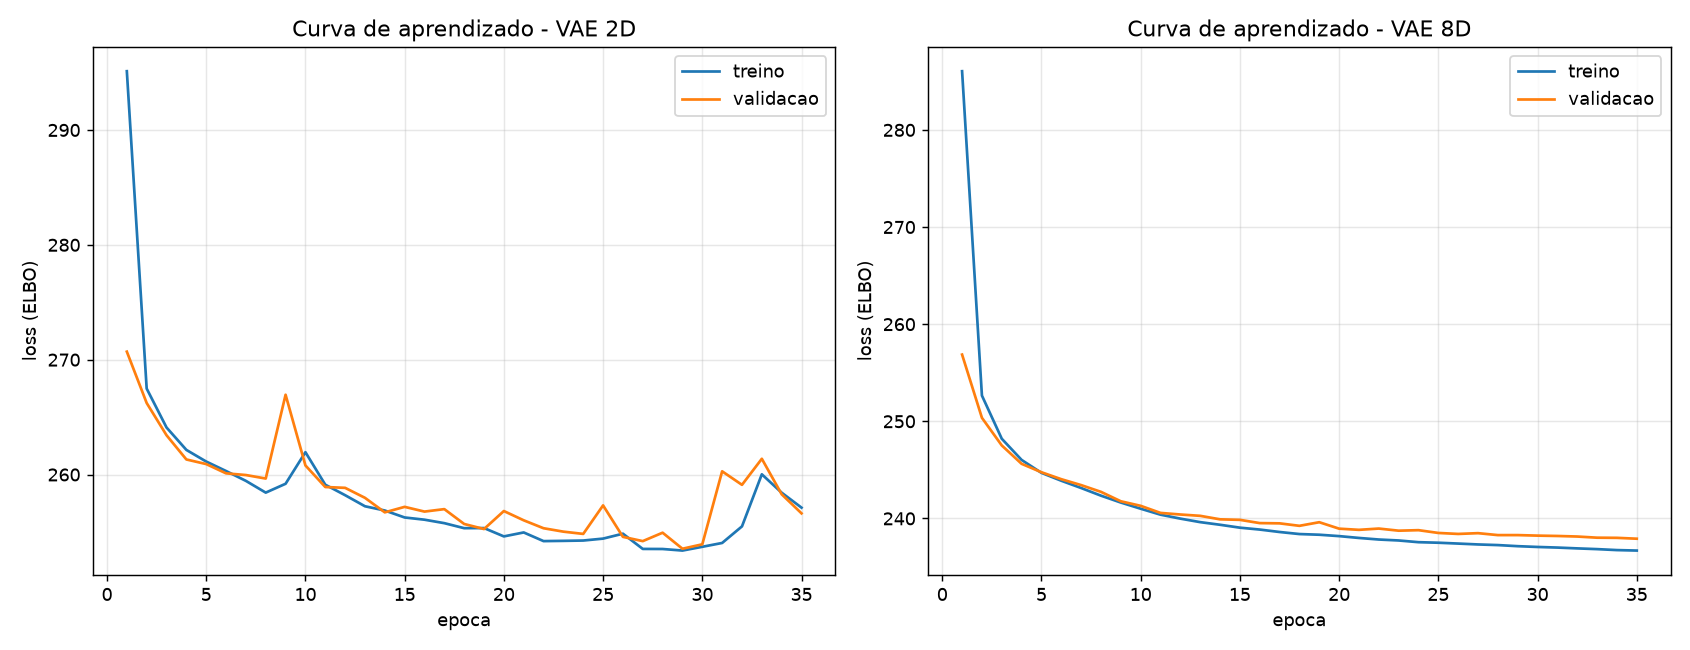
\includegraphics[width=0.92\textwidth]{grafico_curvas_aprendizado_vae.png}
\caption{Curvas de aprendizado (loss ELBO) de treino e validação para os modelos finais 2D e 8D.}
\label{fig:curvas}
\end{figure}

\subsection{Qualidade de reconstrução e geração}
\label{sec:geracao}
As reconstruções (Figuras~\ref{fig:rec2d} e~\ref{fig:rec8d}) confirmam que ambos os modelos capturam a forma das peças; o 8D produz reconstruções visivelmente mais nítidas, consistente com sua menor loss de reconstrução. A prova de que o modelo é \textbf{generativo} está na Figura~\ref{fig:geradas}: amostrando $z \sim \mathcal{N}(0, I)$ e decodificando, obtêm-se peças de vestuário \textbf{novas} e reconhecíveis (camisetas, vestidos, calças, bolsas, calçados) --- que só são plausíveis porque o termo KL deixou o espaço latente próximo da Normal padrão, exatamente a região de onde amostramos.

\begin{figure}[h]
\centering
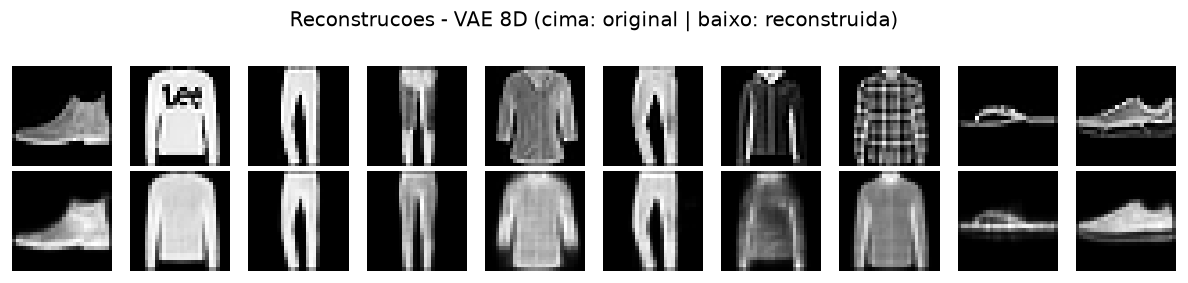
\includegraphics[width=0.85\textwidth]{grafico_reconstrucoes_8d.png}
\caption{Reconstruções do VAE 8D (linha superior: original; inferior: reconstruída) sobre o conjunto de teste.}
\label{fig:rec8d}
\end{figure}

\begin{figure}[h]
\centering
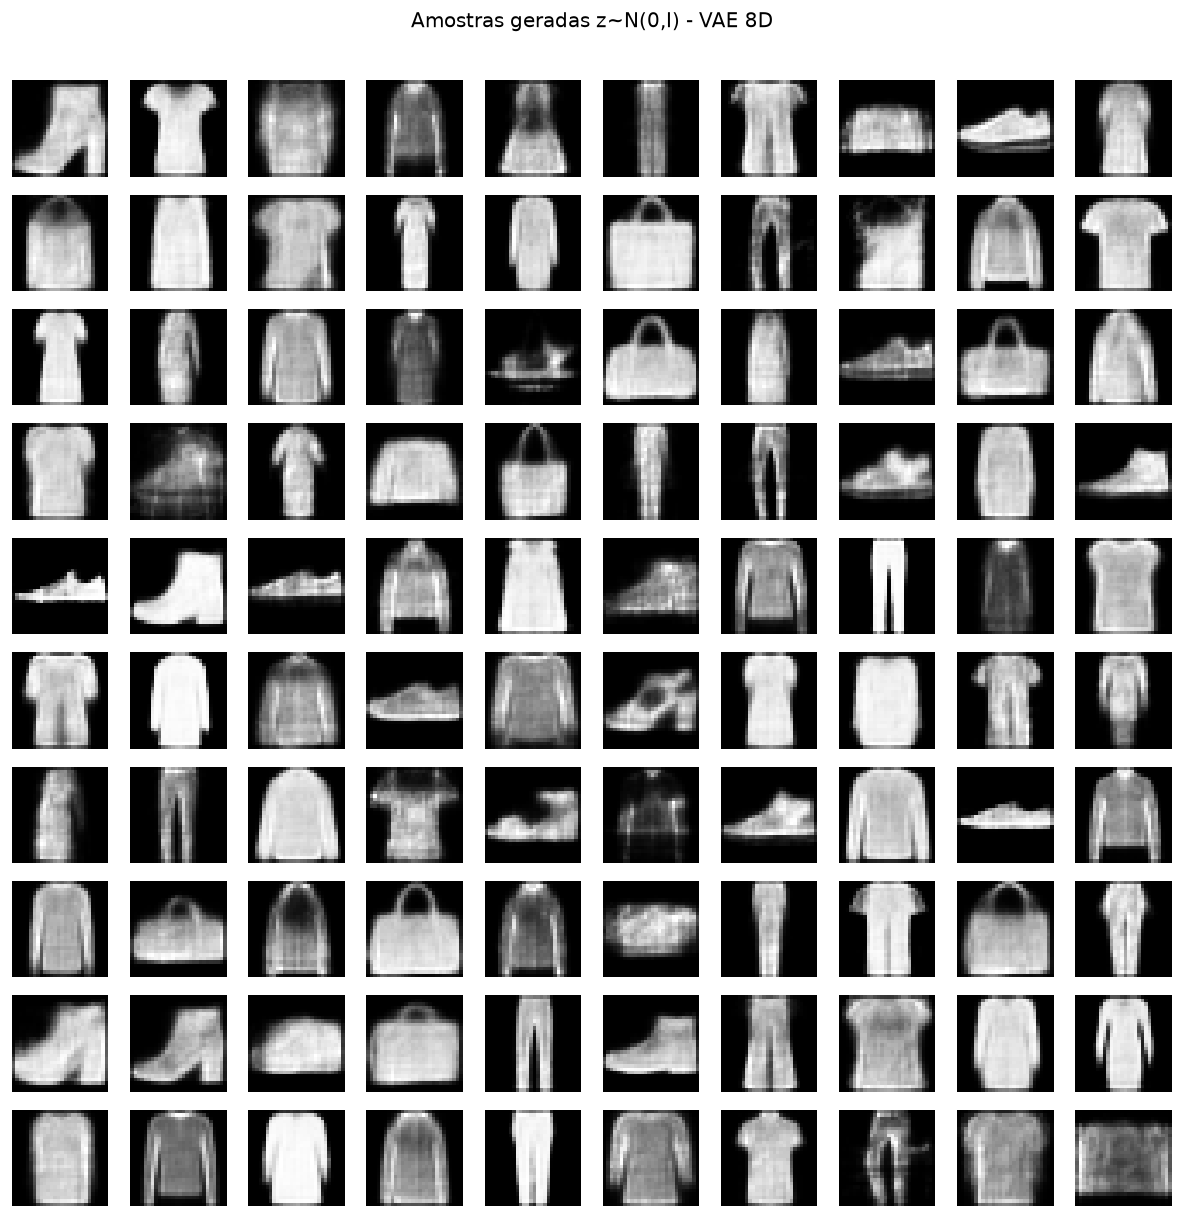
\includegraphics[width=0.52\textwidth]{grafico_amostras_geradas_8d.png}
\caption{Amostras geradas pelo VAE 8D a partir de $z \sim \mathcal{N}(0, I)$: peças de vestuário inéditas (não são cópias do treino).}
\label{fig:geradas}
\end{figure}

\FloatBarrier

\section{Exploração do Espaço Latente}

A Figura~\ref{fig:latente} é o resultado central da exploração: à esquerda, o espaço latente \textbf{2D} do VAE 2D (plotado diretamente, pois já é bidimensional); à direita, a \textbf{projeção PCA} do espaço latente \textbf{8D} em 2D. Em ambos os painéis, os pontos são \textbf{coloridos pelos rótulos} das 10 classes (os rótulos, repita-se, não foram usados no treino).

\begin{figure}[h]
\centering
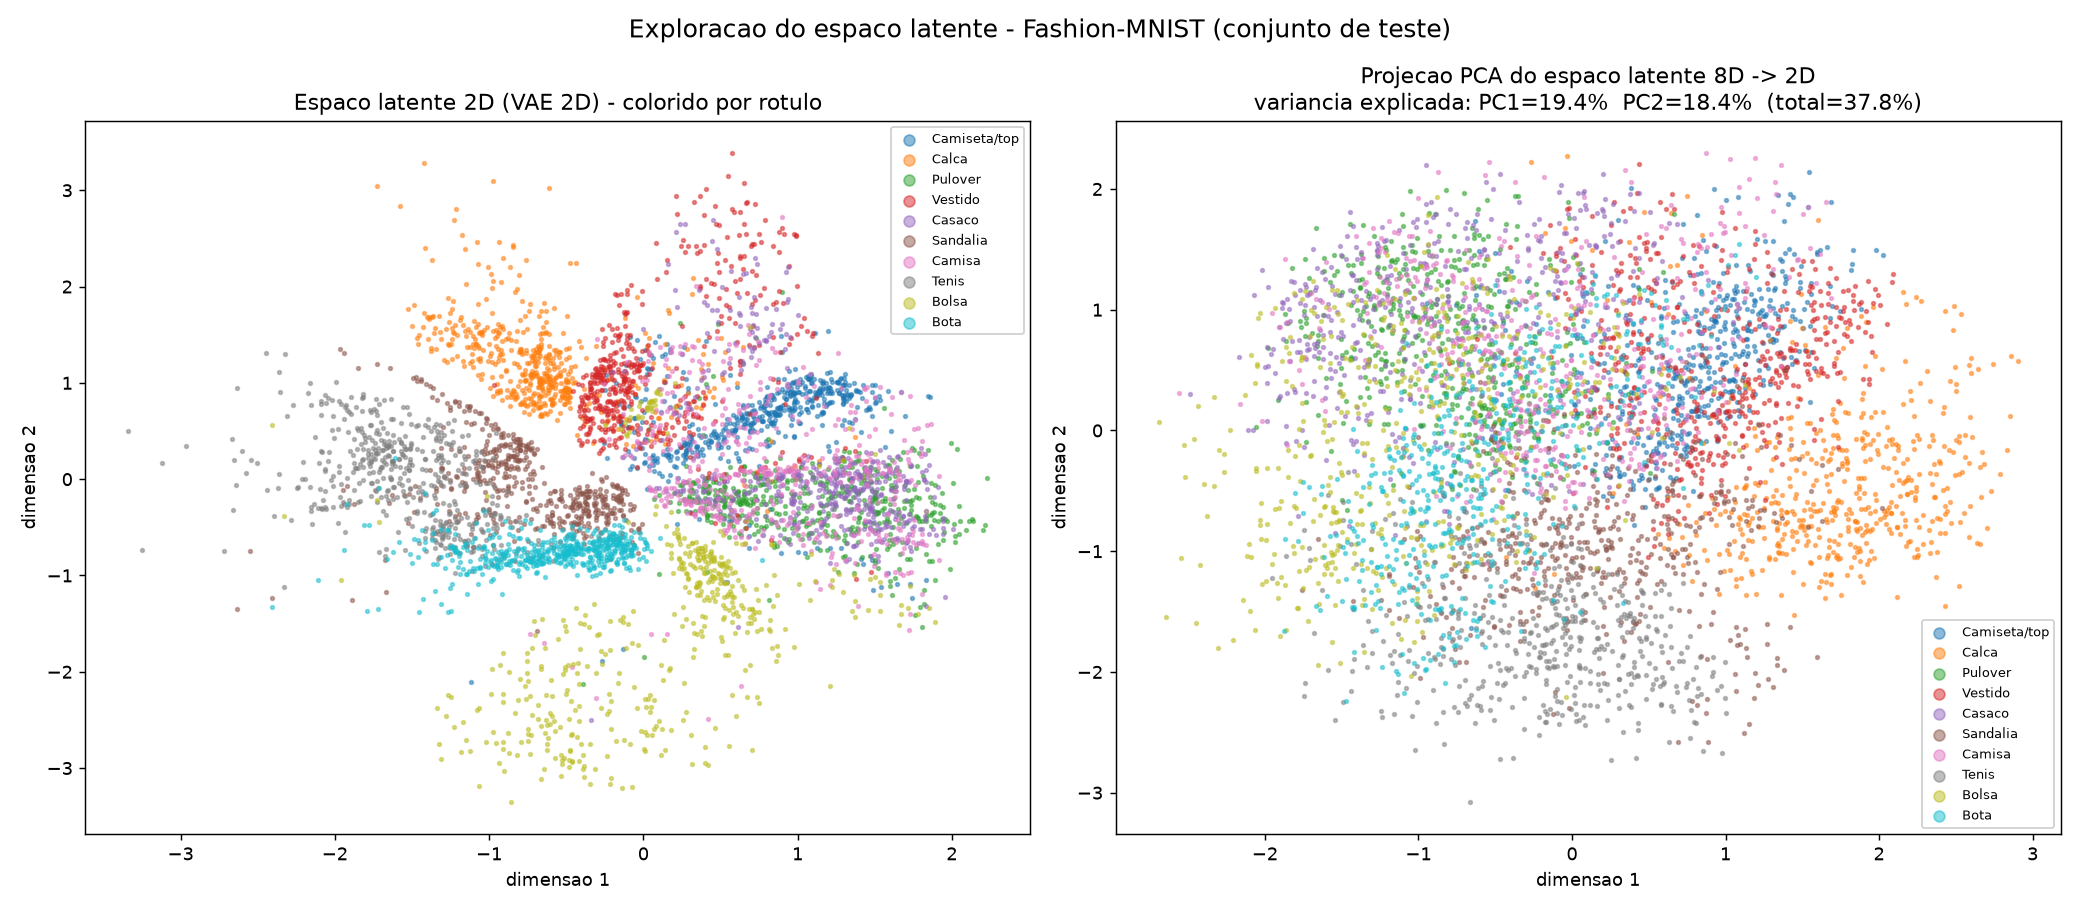
\includegraphics[width=\textwidth]{grafico_espaco_latente.png}
\caption{Exploração do espaço latente (conjunto de teste, colorido por rótulo). Esquerda: espaço latente 2D do VAE 2D. Direita: projeção PCA (8D $\rightarrow$ 2D) do VAE 8D, com a variância explicada por cada componente.}
\label{fig:latente}
\end{figure}

Como o espaço latente 2D é diretamente visualizável, geramos ainda o \textbf{manifold} (Figura~\ref{fig:manifold}): uma grade regular de pontos do plano latente é decodificada, revelando como as peças se transformam \textbf{continuamente} de uma região para outra --- evidência direta de que o espaço é navegável.

\begin{figure}[h]
\centering
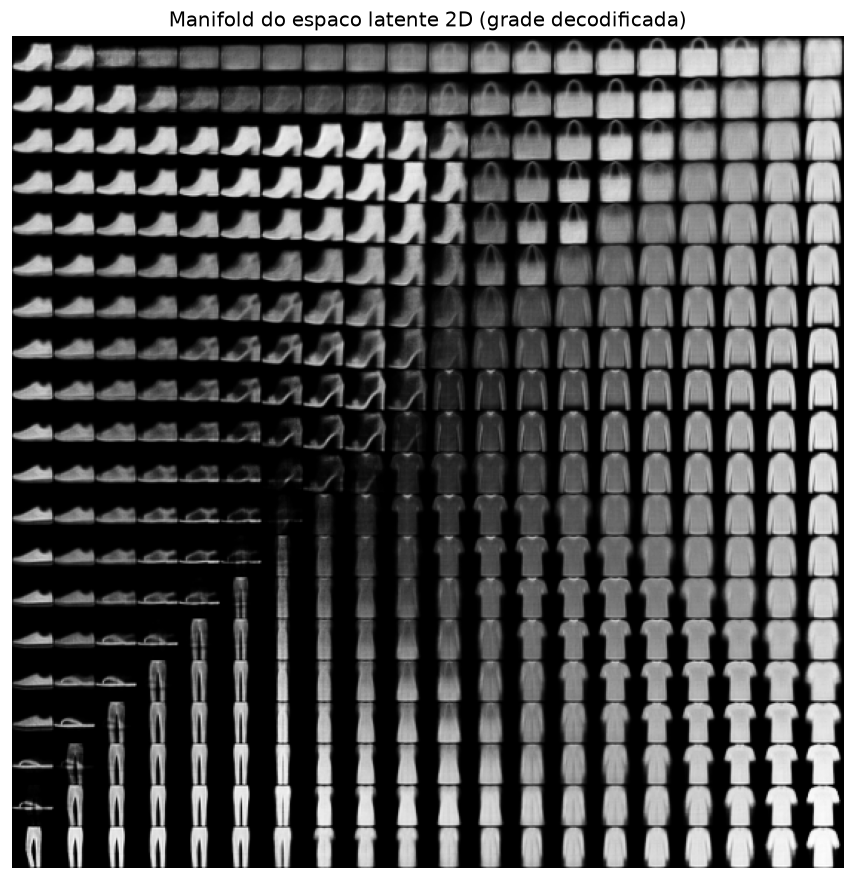
\includegraphics[width=0.6\textwidth]{grafico_manifold_2d.png}
\caption{Manifold do espaço latente 2D: cada célula é a decodificação de um ponto da grade latente. A transição suave entre peças mostra a continuidade do espaço.}
\label{fig:manifold}
\end{figure}

\FloatBarrier

\subsection{Respostas às perguntas do enunciado}

\textbf{(a) Há formação de \textit{clusters} no espaço latente?}
\textbf{Sim.} No espaço latente 2D (Figura~\ref{fig:latente}, esquerda) observam-se agrupamentos nítidos: os \textbf{calçados} (tênis, sandália e bota) ocupam uma região própria à esquerda, a \textbf{bolsa} forma um \textit{cluster} isolado na parte inferior e a \textbf{calça} concentra-se no topo. Isso ocorre mesmo o modelo \textbf{nunca} tendo visto os rótulos --- os agrupamentos emergem da estrutura visual dos dados. Na projeção PCA do 8D há organização por macro-grupos, porém menos separada (ver item c).

\textbf{(b) Há separação dos rótulos no espaço latente?}
\textbf{Parcialmente, e de forma interpretável.} As classes \textbf{visualmente distintas} separam-se bem (calçados, bolsa e calça). Já as classes de \textbf{parte superior do corpo} --- camiseta/top, pulôver, casaco, camisa e vestido --- \textbf{sobrepõem-se} entre si, o que é esperado: são peças genuinamente parecidas em imagens $28\times28$ (um VAE não supervisionado não tem incentivo para separar o que é visualmente semelhante). A sobreposição, portanto, é um resultado coerente, e não uma falha do modelo.

\textbf{(c) A projeção ilustra quanto da variância?}
A projeção PCA do espaço latente \textbf{8D} em 2D explica \textbf{19{,}4\%} (PC1) $+$ \textbf{18{,}4\%} (PC2) $=$ \textbf{37{,}8\%} da variância total. Ou seja, dois componentes capturam pouco mais de um terço da variabilidade dos 8 eixos latentes --- por isso o painel da direita aparece mais ``misturado'' que o da esquerda: cerca de \textbf{62\%} da estrutura do espaço 8D vive em dimensões que a projeção 2D simplesmente não mostra. Isso ilustra bem o compromisso entre \textbf{capacidade} (o 8D reconstrói melhor) e \textbf{visualizabilidade} (o 2D, por já ser bidimensional, é trivialmente mais legível em um gráfico plano).

\section{Conclusões}

Treinou-se com sucesso um VAE generativo para o Fashion-MNIST nas duas configurações pedidas, com topologias selecionadas pela loss de validação e sem vazamento do conjunto de teste. O \textbf{truque da reparametrização} foi o elemento que viabilizou o treino por retropropagação, ao tornar a amostragem latente diferenciável. A exploração confirmou que o espaço latente forma \textbf{clusters} coerentes com as classes (sem jamais usar os rótulos no treino), que a \textbf{separação} é nítida para classes visualmente distintas e esperadamente parcial para as classes de parte superior, e que a projeção PCA do 8D ilustra \textbf{37{,}8\%} da variância --- evidenciando o compromisso entre capacidade latente e facilidade de visualização. Por fim, a geração de peças inéditas a partir de $\mathcal{N}(0, I)$ comprova o caráter generativo do modelo.

\vspace{0.6em}
\hrule
\vspace{0.4em}
{\footnotesize \textit{Observação de reprodutibilidade.} Todos os números e figuras deste relatório foram produzidos por \texttt{vae\_fashion\_mnist\_project3.py} com \textit{Seed}~$=42$. O script detecta automaticamente o dispositivo (CPU ou GPU); os resultados aqui reportados foram obtidos em CPU com 35 épocas de re-treino final e busca de 8 épocas por configuração. Pequenas variações numéricas podem ocorrer entre diferentes versões de bibliotecas ou \textit{hardware}.}

\end{document}
